\documentclass[11pt,a4paper]{article}
\usepackage[paper=a4paper,left=25mm,right=20mm,top=30mm,bottom=30mm]{geometry} 
\usepackage[english, ngerman]{babel}
\usepackage[utf8]{inputenc}
\usepackage[colorlinks=false]{hyperref}
\usepackage[table,usenames,dvipsnames]{xcolor}
\usepackage{tabularx}
\usepackage{graphicx}
\usepackage{subfigure}
\usepackage{listings}
\usepackage{float}
\usepackage{hyperref}
\usepackage{multicol}
\usepackage{fancyhdr}
\usepackage{sectsty}
\usepackage[final]{pdfpages}
\usepackage{threeparttable}
\usepackage{amsmath}
\usepackage{tikz}
%\usepackage{gitinfo}
\usepackage{totpages}
\usepackage{datetime}
\usepackage[printonlyused]{acronym}
%\usepackage{syntonly}
%\syntaxonly
  
%Definitionen
\includepdfset{pages=-} %Alle Seite importieren  Option: noautoscale
\setlength{\parindent}{0em} %Einrueckung eines neuen Absatzes, 0 keine Einrueckung

\definecolor{rowc1}{RGB}{40,75,95}

\setcounter{tocdepth}{3}
\setcounter{secnumdepth}{3}

\ifpdf
\pdfinfo {
	/Author (Marc Schärer, Arthur van Ommen, Fabian Affolter)
	/Title (Report)
	/Subject ()
	/Keywords ()
	/CreationDate (D:\pdfdate)
}
\fi

\pagestyle{fancy}
\renewcommand{\headrulewidth}{0pt}
\lhead{}%\includegraphics[width=80mm]{logo.png}}
\chead{}
\rhead{}
\lfoot{}
\cfoot{\thepage}
\rfoot{}

\definecolor{mygreen}{rgb}{0,0.6,0}
\definecolor{mygray}{rgb}{0.5,0.5,0.5}
\definecolor{mymauve}{rgb}{0.58,0,0.82}

\lstset{ %
  backgroundcolor=\color{white},   % choose the background color; you must add \usepackage{color} or \usepackage{xcolor}
  basicstyle=\footnotesize,        % the size of the fonts that are used for the code
  breakatwhitespace=false,         % sets if automatic breaks should only happen at whitespace
  breaklines=true,                 % sets automatic line breaking
  captionpos=b,                    % sets the caption-position to bottom
  commentstyle=\color{mygreen},    % comment style
  deletekeywords={...},            % if you want to delete keywords from the given language
  escapeinside={\%*}{*)},          % if you want to add LaTeX within your code
  extendedchars=true,              % lets you use non-ASCII characters; for 8-bits encodings only, does not work with UTF-8
  frame=single,                    % adds a frame around the code
  keepspaces=true,                 % keeps spaces in text, useful for keeping indentation of code (possibly needs columns=flexible)
  keywordstyle=\color{blue},       % keyword style
  language=Octave,                 % the language of the code
  morekeywords={*,...},            % if you want to add more keywords to the set
  numbers=left,                    % where to put the line-numbers; possible values are (none, left, right)
  numbersep=5pt,                   % how far the line-numbers are from the code
  numberstyle=\tiny\color{mygray}, % the style that is used for the line-numbers
  rulecolor=\color{black},         % if not set, the frame-color may be changed on line-breaks within not-black text (e.g. comments (green here))
  showspaces=false,                % show spaces everywhere adding particular underscores; it overrides 'showstringspaces'
  showstringspaces=false,          % underline spaces within strings only
  showtabs=false,                  % show tabs within strings adding particular underscores
  stepnumber=2,                    % the step between two line-numbers. If it's 1, each line will be numbered
  stringstyle=\color{mymauve},     % string literal style
  tabsize=2,                       % sets default tabsize to 2 spaces
  title=\lstname                   % show the filename of files included with \lstinputlisting; also try caption instead of title
}

\renewcommand{\arraystretch}{1.3}

\lstset{basicstyle=\ttfamily,breaklines=true}

\begin{document}
%PRE DOCUMENT STUFF%%%%%%%%%%%%%%%%%%%%%%%%%%%%%%%
\definecolor{titlepagecolor}{RGB}{40,75,95}
\DeclareFixedFont{\titlefont}{T1}{ppl}{b}{}{0.5in}

\makeatletter
%%%%%%%%%%%%%%%%%%%%%%%%%%%%%%%%%%%%%%%%%%%%%%%%%%%%%%%%%%%%%%%%%%%%%%%%%%%%%%
\def\printfooterline{\begin{scriptsize}
Datum: {\today} -- 
Seiten: \ref*{TotPages}  -- 
Version: 1.0, \gitAbbrevHash
\end{scriptsize}
}
\def\printtitle{
% Title
\titlefont{Hochregallager}\par
\vspace{20pt}
%Sub title
{\LARGE Modellierung und Simulation}\par
\vspace{100pt}
{\Large    }\par
}
\def\printauthor{%                  
    {\large \@author}}              
\makeatother
\def\authorshort{Fabian Affolter}
\author{%
    Berner Fachhochschule - Technik und Informatik \vspace{10pt}\\
    Marc Schärer 
    \href{mailto:scham36@bfh.ch}{scham36@bfh.ch} \\
    Arthur van Ommen 
    \href{mailto:vanoa1@bfh.ch}{vanoa1@bfh.ch} \\
    Fabian Affolter 
    \href{mailto:affof1@bfh.ch}{affof1@bfh.ch} \\
    }
%%%%%%%%%%%%%%%%%%%%%%%%%%%%%%%%%%%%%%%%%%%%%%%%%%%%%%%%%%%%%%%%%%%%%%%%%
% The following code is borrowed from: http://tex.stackexchange.com/a/86310/10898

\newcommand\titlepagedecoration{%
\begin{tikzpicture}[remember picture,overlay,shorten >= -10pt]

\coordinate (aux1) at ([yshift=-15pt]current page.north east);
\coordinate (aux2) at ([yshift=-410pt]current page.north east);
\coordinate (aux3) at ([xshift=-4.5cm]current page.north east);
\coordinate (aux4) at ([yshift=-150pt]current page.north east);

\begin{scope}[titlepagecolor!40,line width=12pt,rounded corners=24pt]
\draw
  (aux1) -- coordinate (a)
  ++(225:5) --
  ++(-45:5.1) coordinate (b);
\draw[shorten <= -10pt]
  (aux3) --
  (a) --
  (aux1);
\draw[opacity=0.6,titlepagecolor,shorten <= -10pt]
  (b) --
  ++(225:2.2) --
  ++(-45:2.2);
\end{scope}
\draw[titlepagecolor,line width=8pt,rounded corners=14pt,shorten <= -10pt]
  (aux4) --
  ++(225:0.8) --
  ++(-45:0.8);
\begin{scope}[titlepagecolor!70,line width=6pt,rounded corners=14pt]
\draw[shorten <= -10pt]
  (aux2) --
  ++(225:3) coordinate[pos=0.45] (c) --
  ++(-45:3.1);
\draw
  (aux2) --
  (c) --
  ++(135:2.5) --
  ++(45:2.5) --
  ++(-45:2.5) coordinate[pos=0.3] (d);   
\draw 
  (d) -- +(45:1);
\end{scope}
\end{tikzpicture}%
}

\begin{titlepage}
\noindent
\printtitle
\null\vfill
\vspace*{1cm}
\noindent
\hfill
\begin{minipage}{0.6\linewidth}
    \begin{flushright}
        \printauthor
    \end{flushright}
\end{minipage}
%
\begin{minipage}{0.02\linewidth}
    \rule{1pt}{125pt}
\end{minipage}
\titlepagedecoration
\vspace{20pt}
\begin{minipage}{0.9\linewidth}
%\printfooterline
\end{minipage} 
\end{titlepage}


\pagenumbering{Roman} % Seitennummerierung durch roemische Ziffern
\renewcommand{\contentsname}{Inhaltsverzeichnis}
\tableofcontents

%%\begin{abstract}
\section*{Zusammenfassung}
%
Das Hochregallager ist ein Lagerungssystem, welche sich mit einer hohen Lagerdichte und Wirtschaftlichkeit von anderen Konzepten abhebt...\newline


%
% %EOF

\pagenumbering{arabic} % Seitennummerierung durch arabische Ziffern
\clearpage

%%%%%%%%%%%%%%%%%%%%%%%%%%%%%%%%%%%%%%%%%%%%%%%%%
\section{Einleitung}
Ein Hochregallager (HRL) beschreibt ein Lagersystem mit Plätzen in sogenannten Regalen. Hochregallager gibt ein in den unterschiedlichsten Ausprägungen. Die grössten Ausführungen besitzen Höhen bis etwa 50 m und können mehreren hunderttausend Plätze besitzen. Oftmals werden direkt Euro-Paletten als Träger für das Lagergut verwendet, ist das Lagergut zu klein, werden häufig spezielle Kunststoff-Behälter benutzt.\\
Grobgesagt besteht ein Hochregallager aus einer bestimmten Anzahl von Gassen. Eine Gasse wiederum hat links und rechts Lagerplätze und im Freiraum bewegt sich ein Bediengerät. In einem manuellen Hochregallager ist dieser Raum so gross, dass mit einem Gabelstapler zwischen den Regalwänden manövriert werden kann. Bei automatischen Lagern fährt ein Bediengerät, welches von einem Lagerverwaltungssystem seine Befehle bekommt, ohne manuelle Interventionen in der Gasse und liefert das Lagergut zur Entnahmestelle.\\
Die Hochregallager haben eine hohe Raumnutzung und bei der Erstellung sind hohe Investitionen nötig, da bei kleiner Ausführungen eine Halle um das Hochregallager gebaut werden muss. Bei grossen Varianten wird das Hochregal als Tragstruktur für das Gebäude mitbenutzt.\\
Dieses Dokument beschreibt in stark reduzierter Form die wichtigsten Aspekte der Anwendung. Die Installations- und Benutzungsanleitung ist separat verfügbar.
%
\subsection{Rahmenbedingungen}
Die verwendete Programmiersprache ist Java. Die Abgabe des Projektes ist in der letzten Woche des Herbstsemester 2013/2014.
%
\subsection{Abgrenzung}
Die Schnittstelle liegt an der Stirnseite des Hochregallagers zur Vorzone. Die gestrichelte Linie in \ref{fig:overview} auf Seite \pageref{fig:overview} stellt diese Grenze dar. Das Hochregal hat keine fest definierte Abmessungen und auch die Lagergüter habe keine definierten Masse oder Gewicht. Es wird davon ausgegangen, dass die Lagergüter auf einem Träger (z. B. Euro-Palette) platziert sind oder sich in einem Behälter befinden und so zum Hochregal kommen. Alle Lagergüter werden mit den gleichen physikalischen Bedingungen befördert.\\ 
%EOF

\section{Grundlagen}
Im Sinne eines Hochregallager besteht eine Gasse aus einer rechten und einer linken Regalwand während sich in der Mitte der beiden Wände ein Korridor für das Regalbediengerät (RBG) befindet. Die Regalwände sind in Lagerplätze unterteilt, die von Regalbediengerät be- und entladen werden. Hochregallager können aus einer beliebigen Anzahl Gassen bestehen. Im Normalfall befindet sich an einer Stirnseite der Gassen die sogenannte Vorzone, welche die Aufgabe hat, die Lagergüter auf die zugeweisen Gassen zu verteilen. 
%
\begin{figure}[H]
  \begin{center}
    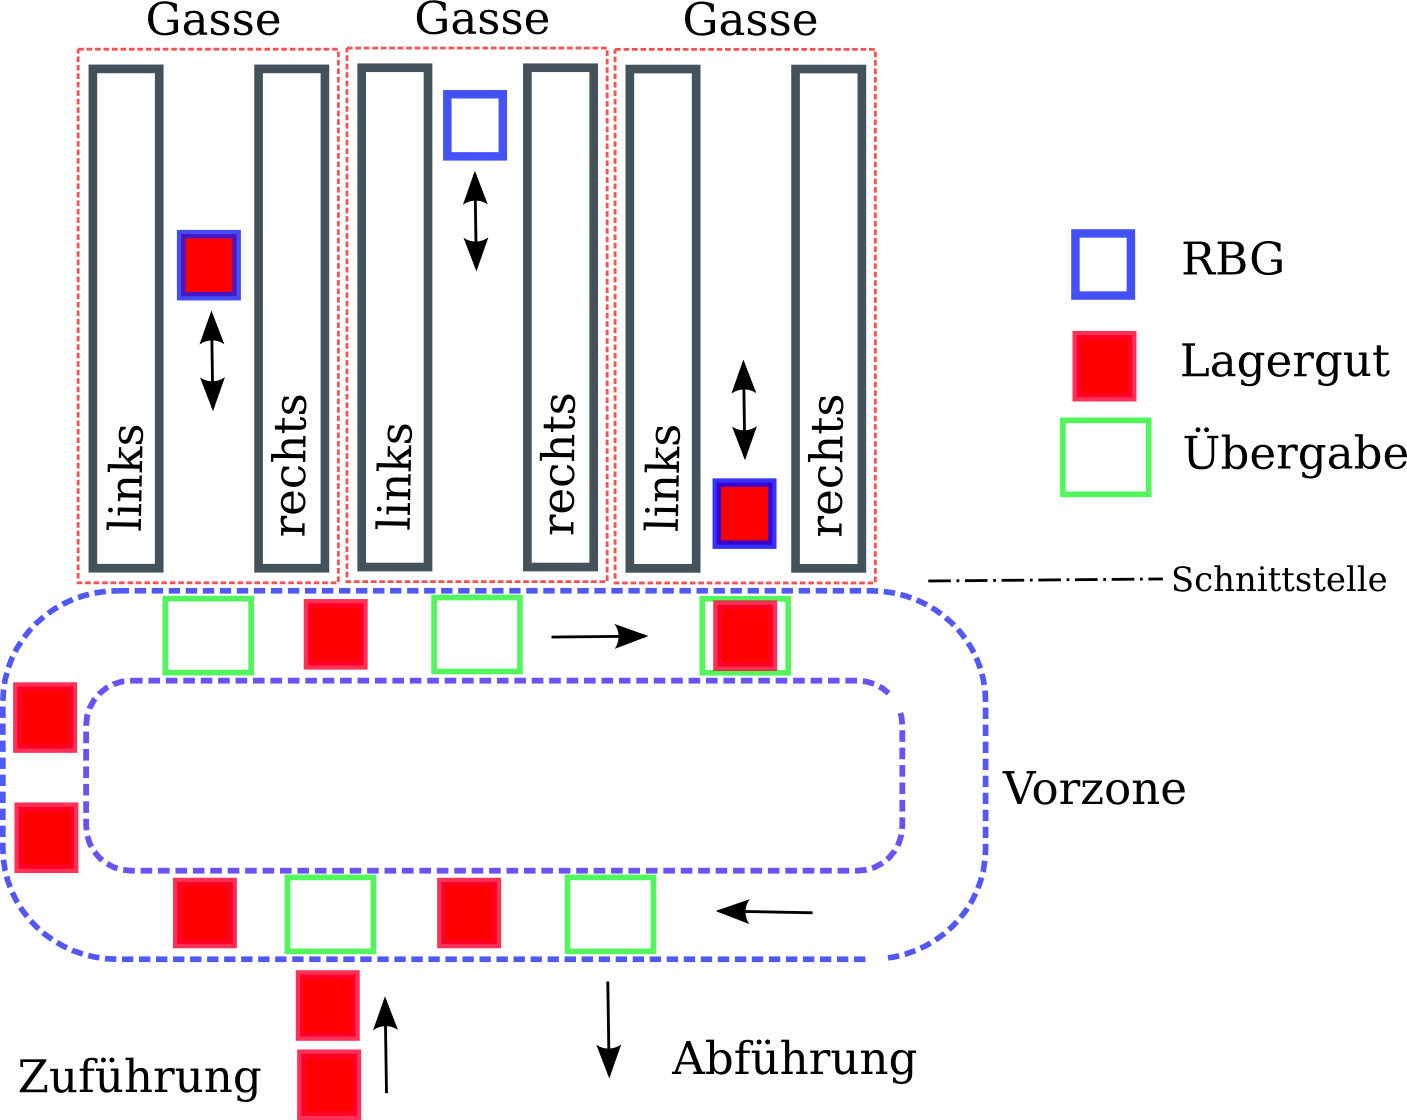
\includegraphics[width=0.8\textwidth]{images/uebersicht.png}
    \caption{Übersicht}
    \label{fig:overview}
  \end{center}
\end{figure}
%

%
\subsection{Allgemeine Grundlagen}
Dieser Abschnitt enthält Details allgemeiner Natur, damit im weiteren Verlauf des Dokuments Unklarheiten vermieden werden können. Die Sprache innerhalb des Source Code ist Englisch, während die Dokumentationssprache Deutsch ist. Die wichtigsten Benennungen sind in \ref{tab:desc} ersichtlich.
%
\begin{table}[H]
  \caption{Benennungen}
  \label{tab:desc}

  \begin{center}
    \begin{tabular}{cc}
       Location & Lager\\
       Gap & Gasse\\
       Grid & Regalwand \\
       Column & Spalten im Regal \\
       Row & Zeilen im Regal \\
       Bin & Lagerfach \\
       Rack feeder & Regelbediengerät \\
    \end{tabular}
  \end{center}
\end{table}
%
\subsubsection{Koordinaten}
Der Koordinatenursprung befinet sich in der linken unteren Ecke der Regalwand (Grid). Es wird yz-Koordinatensystem aufgespannt und die Koordinaten der Lagerplätze (Bins) sind in die linke untere Ecke gesetzt. Das Regalbediengerät kann sich auf der y- und der z-Achse bewegen. Der Übergabebereich befindet sich ausserhalb des Koordinatensystems auf dem negativen Abschnitt der y-Achse. 
%
\begin{figure}[h]
  \begin{center}
    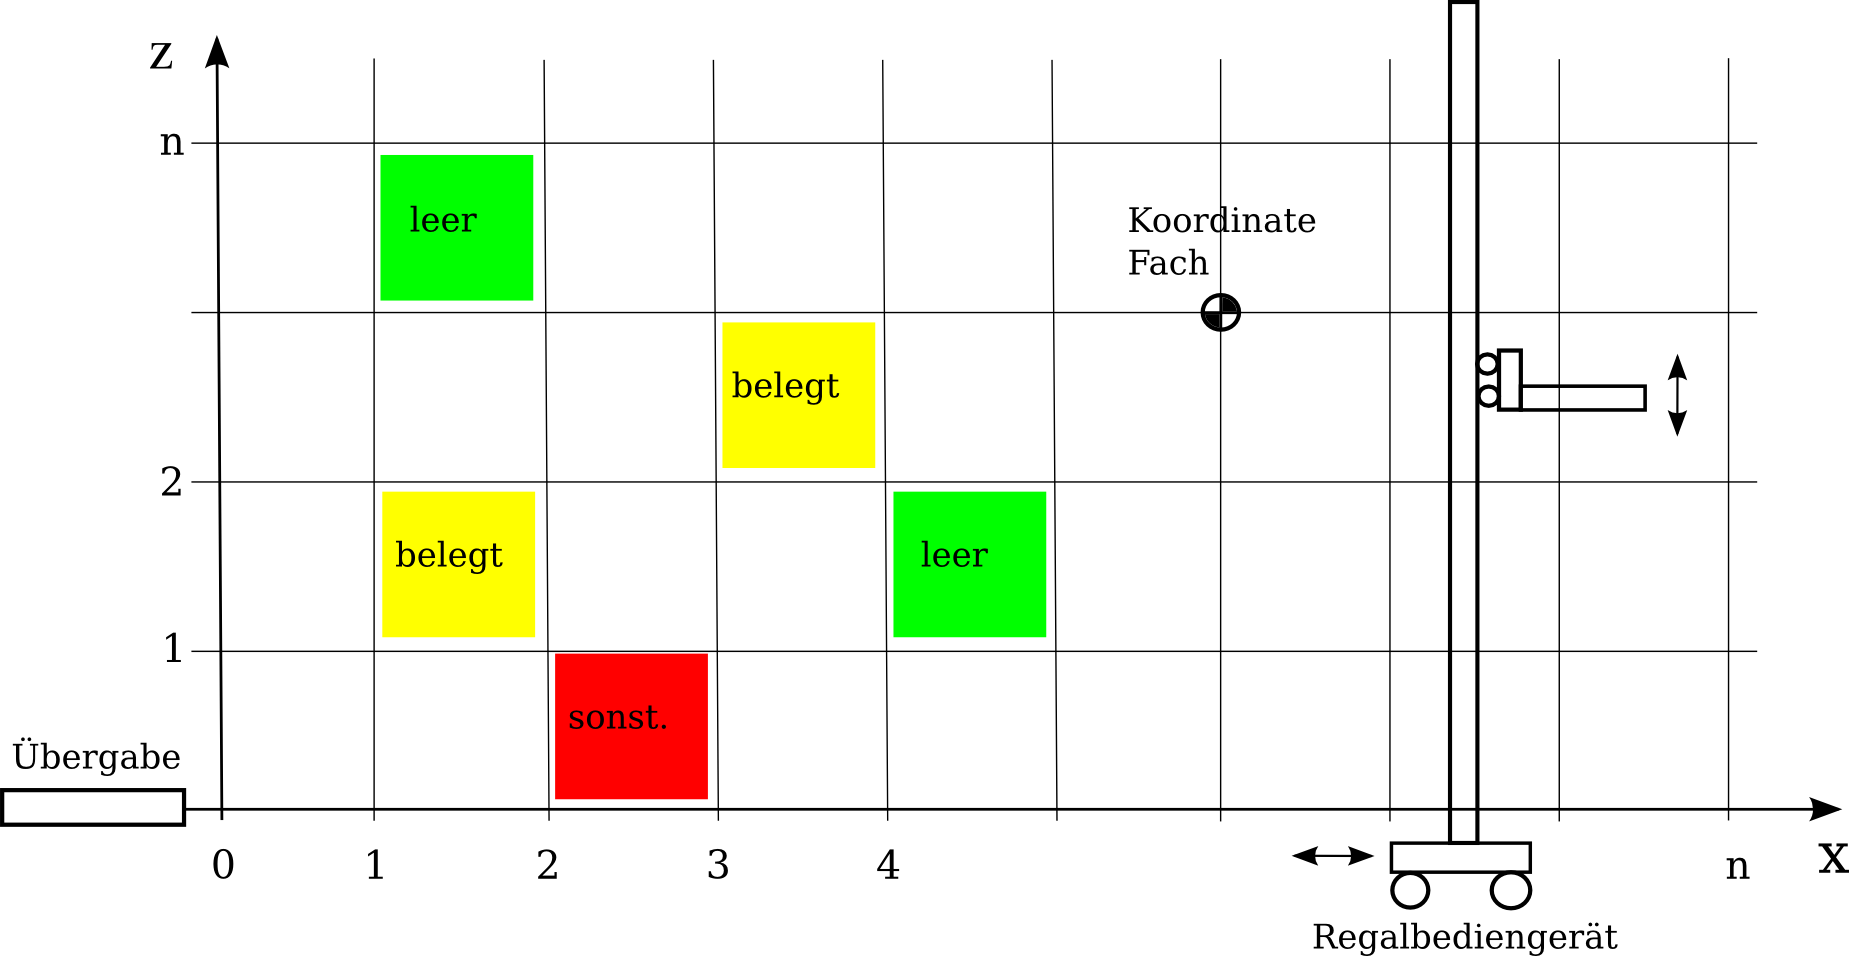
\includegraphics[width=0.9\textwidth]{images/koordinaten-wand.png}
    \caption{Lagerwand}
    \label{fig:wand}
  \end{center}
\end{figure}
%
In Abbildung \ref{fig:wand} sind ebenfalls die verwendete Farbzuordung für die Lagerplätze (Bins) ersichtlich.
%
\begin{table}
  \caption{Farbzuordung Lagerplätze}
  \label{tab:bin-color}

  \begin{center}
    \begin{tabular}{cc}
       grün & leer\\
       gelb & belegt\\
       rot & reserviert/defekt/spezial (wird nicht implementiert) \\
    \end{tabular}
  \end{center}
\end{table}

%
\subsubsection{Klappung}
Für die zweidimensionale Darstellung wird eine Lagergasse gemäss Abbildung \ref{fig:klapp} aufgefaltet, respektive aufgeklappt. Dies erlaubt die komplette Darstellung einer Lagergasse. In der Visualisierung ist die Gasse so dargestellt. Dies ist dehalb wichtig, da sich die Achsen des Koordinatensystems entsprechend der Klappung ändern.  
%
\begin{figure}[H]
  \begin{center}
    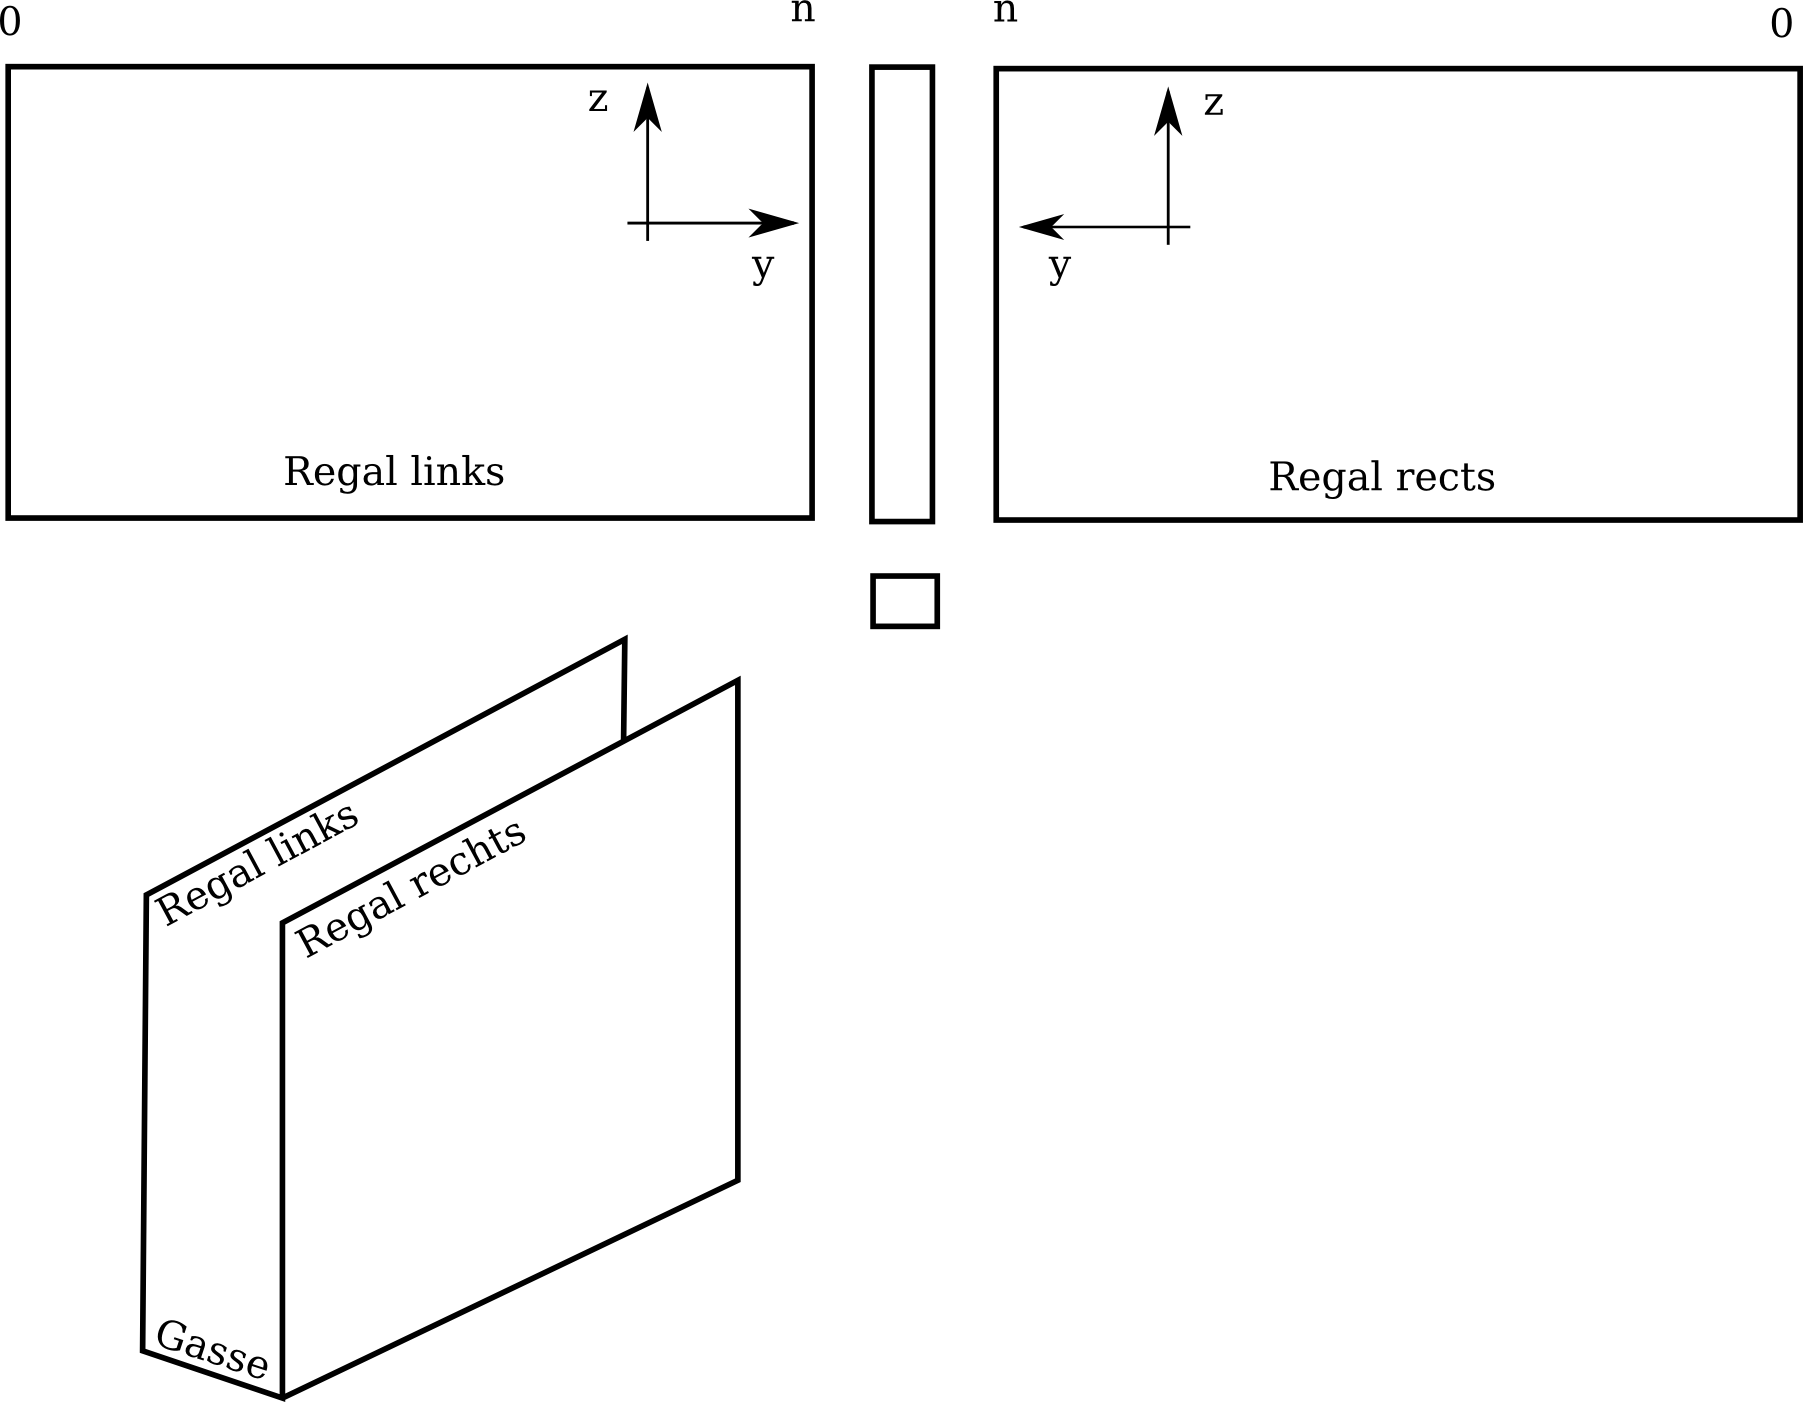
\includegraphics[width=0.7\textwidth]{images/klappung.png}
    \caption{Klappung}
    \label{fig:klapp}
  \end{center}
\end{figure}

%
\subsection{Mathematische Grundlagen}
Das Regalbediengerät bewegt sich in der Gasse zwischen den Lagerwänden auf der y- und der z-Achse. Der Arm des Regalbediengerät verfährt auf der y-Achse und der Ausleger auf der z-Achse. Die Bewegungen auf beiden Achsen lassen somit entsprechend der elektromechanischen Steuerung beliebige Verfahrwege auf der yz-Ebene zu. Die Graduierung der Bewegungsbahn wird durch die Grösse der Inkremente bestimmt.
%
Die Grundgleichung für die Geschwidigkeit in der Ebene lautet:
%
\begin{equation}
v = \frac{s}{t}
\end{equation}
%
Die Fahrt des Regalbediengerät besteht aus einer Phase für die Beschleunigung, einer Phase der gleichförmigen Bewegung mit möglichst maximaler Geschwindigkeit und einem Bremsabschnitt, resp. einer Verzögerungsphase, am Ende. In allen Berechnung wird die Masseträgheit des Regalbediengerätes vernachlässigt. Die Einflüsse durch die Masse der Lagergüter auf die Dynamik des Regalbedientgerätes wird nicht untersucht oder in den Berechnungen berücksichtigt. Die Annahme ist, dass die Lagergüter masslos sind und bei Beschleugigung und Verzögerung weder kippen noch verrutschen können. Weiter führt die Vernachlässigung der Ergbeschleunigung bei Bewegungen auf der z-Achse zu Fehler. Die Erdbeschleuigung ($ g $) summiert sich bei einer Bewegung in Richtung der negativen z-Achse zur vorhandenen Beschleunigung hinzu und bei Bewegungen in positiver Richtung (nach oben) müsste sie zusätzlich überwunden werden. Das Regalbediengerä wird als reibungfrei angenommen.
%
Die kürzeste Fahrzeit ergibt sich auch mehreren Faktoren. Die Synchronisationsgerade ist ein in diesem Zusammenhang oft verwendeter Begriff, welcher die optimale Fahrbahn des Regalbediengerät beschreibt. Dieser Fahrbahn führt jedoch nicht zur optimalen Fahrzeit, da unter Umständen auf beide Achsen gebremst werden müssten. Wir haben den Ansatz gewählt, dass, wenn möglich, nur auf der schnelleren Achse die Geschwindigkeit reduziert wird, was dazuführt, dass sich die zweite Achse entsprechend ihrem Maximum fortbewegen kann.
%
Ein Grenzfall tritt auf, wenn die zu bewältigende Strecke kleiner wird als die Summe der Wege von der Beschleunigung und Verzögerung bei konstanten Beschleunigungen/Verzögerungen und Geschwindigkeiten. 
%
\begin{equation}
v = \sqrt{\frac{2 \cdot s \cdot a \cdot d}{(a+d)}}
\end{equation}
%
\subsection{Simulationstechnische Grundlagen}
%




%EOF


\section{Modellierung}
Der Aufbau des Hochregallagers wurde in diverse Bereiche unterteilt. Die wichtigsten sind das Hochregal selber, auch auch das Regalbediengerät und und die entsprechenden Zustände/Ereignisse, die innerhalb des Hochregallagers auftreten können. 
%
\subsection{Einheiten}
Die Basiseinheit ist Milimeter. Es ist jedoch möglich mit anderen SI-Einheiten (m, dm oder cm) zu arbeiten.
%
\subsection{Hochregal}
Das gesamt Hochregallager wird durch ein einzelnes Objekt dargestellen. Dieses Objekt enthält alle benötigten Informationen. Das heisst, dass auf die Gassen, das Regal und die Lagerfächer direkt zugegriffen werden kann. Dies biete eine komfortables Arbeiten bei der Simulation. Weiter bietet es den Vorteil, dass alle Informationen über die Elemente des Lagerortes immer verfügbar sind und abgefragt werden können.
%
\subsection{Regalbediengerät}
Innerhalb der Gasse bewegt sich nur das Regalbediengerät. Die Klasse RackFeeder bildet dies ab. In vorherigen Abschnitt wurde auf die zulässigen Bewegungen eingegangen. Die maximalen Beschleuigungen, Verzögerungen und die Geschwindigkeit sind innerhalb dieses Klasse als Standwerte definiert. Bei Bedarf lassen sie sich überschreiben. Das Regalbediengerät 
%
\subsection{Ereignisse}
Innerhalb des Systems wurden die Ereignisse (Events) in die Operationen Einlagern, Umlagern und Auslagern zerlegt. Die Verzweigungen sind in den nachfolgenden Abbildungen in gelb dargestellt. Der Startpunkt ist blau. 
%
% Im Verhalten Einlagern
% 
% 1.1 RBG auf 0/0 leer
% 2 RBG auf 0/0 beladen
% 3 RBG auf Y/Z beladen
% 4 RBG auf X beladen
% 5 RBG auf X leer
% 6 RBG auf Y/Z leer
% 1.2 RBG auf 0/0 leer
% 
% Im Verhalten Auslagern
% 
% 1.1 RBG auf 0/0 leer
% 6 RBG auf Y/Z leer
% 5 RBG auf X leer
% 4 RBG auf X beladen
% 3 RBG auf Y/Z beladen
% 2 RBG auf 0/0 beladen
% 1.2 RBG auf 0/0 leer
% 
% Nachfolgendens Entladen
% 
% 7 RBG auf Y1/Z1 leer -> dann in normalen Entlade-Zuklus
% 
% Im Verhalten Umlagern
% 
% 6 RBG auf Y/Z leer
% 5 RBG auf X leer
% 4 RBG auf X beladen
% 3 RBG auf Y/Z beladen
% 8 RBG neues Lagerfach !!
% 3 RBG auf Y/Z beladen
% 4 RBG auf X beladen
% 5 RBG auf X leer
% 6 RBG auf Y/Z leer -> 7 oder 1
% 
% Änderungen
% 7 und 8
%
\begin{figure}[H]
  \begin{center}
    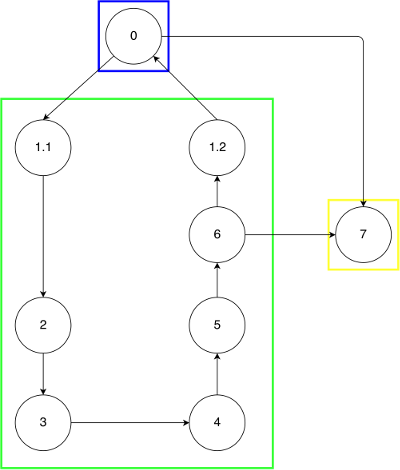
\includegraphics[width=0.3\textwidth]{images/einlagern.png}
    \caption{Einlagern}
    \label{fig:in}
  \end{center}
\end{figure}
%
\begin{figure}[H]
  \begin{center}
    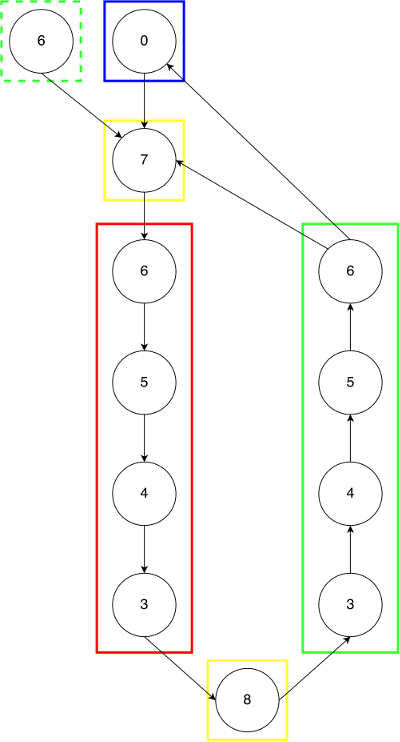
\includegraphics[width=0.3\textwidth]{images/umlagern.png}
    \caption{Umlagern}
    \label{fig:move}
  \end{center}
\end{figure}
%
\begin{figure}[H]
  \begin{center}
    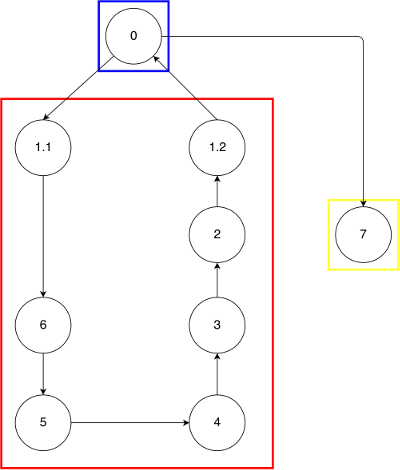
\includegraphics[width=0.3\textwidth]{images/auslagern.png}
    \caption{Auslagern}
    \label{fig:out}
  \end{center}
\end{figure}
%

\subsection{Zustände}

\subsubsection{Global}
\begin{enumerate}
  \item Get next free Gap
  \item Select Gap (first to be free?)
  \item .1 Assign Item to Bin
  \item .2 Send Item to Gap
  \item .3 Set RBG to 0.0
  \item Load Item to RBG
  \item Store Item in Bin
\end{enumerate}
%
\subsubsection{Gassen}

\paragraph{RBG Einlagern}

\begin{table}[H]
  \caption{Einlagerung}
  \label{tab:ins}

  \begin{center}
    \begin{tabular}{ccc}

		Eventnr.	& Koord.	& Zustand \\
		\hline
		1 &			0/0 	& empty\\
		2 &			0/0 	& loaded\\
		3 &			y/z 	& loaded\\
		4 	&		x 		& loaded\\
		5 &			x 		& empty\\
		6 &			y/z 	& empty\\
		1	&		0/0		& empty\\
		7 &					& sleep\\
    \end{tabular}
  \end{center}
\end{table}	
\paragraph{RBG Auslagern}

\begin{table}[H]
  \caption{Auslagerung}
  \label{tab:outs}

  \begin{center}
    \begin{tabular}{ccc}
		Eventnr.&	Koord.&	Zustand\\
		\hline
		1 &			0/0 	&empty\\
		6 &			y/z 	&empty\\
		5 &			x 		&empty\\
		4 &			x 		&loaded\\
		3 &			y/z 	&loaded\\
		2 &			0/0 	&loaded\\
		1	&		0/0		&empty\\
		7 &					&sleep \\
    \end{tabular}
  \end{center}
\end{table}	
%
\subsection{Bewegungen}



%
\subsection{Steuer-Daten}

%
\subsection{Architektur}
Die Unterteilung der Anwendung erfolgte in einen Teil für die Modellierung, Simulation und die Visualisierung.  





%EOF

\section{Simulation}



%EOF

\section{Visualisierung}
Auf Grund der hohen Dichte von möglichen Visualisierungselementen wird das Hochregallager aufgeklappt und  vvereinfacht dargestellt.

%
\subsection{Trennung}
Der Lagerwand und den involvierten Akteure wurde je eine Ebene (Layer) zugeweisen. Dies stellt sicher, dass bei der Darstellung nur die Elemente, welche sich seit dem letzten Schritt verändert haben, neugeladen werden müssten.  

%
\begin{figure}
\subfigure[Lagergitter]{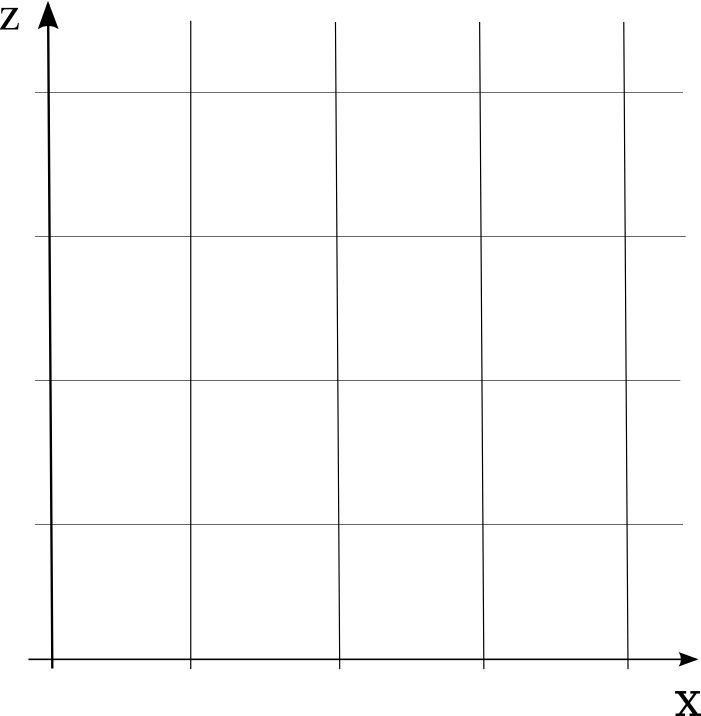
\includegraphics[width=0.29\textwidth]{images/lagergitter.png}}\hfill
\subfigure[Belegung]{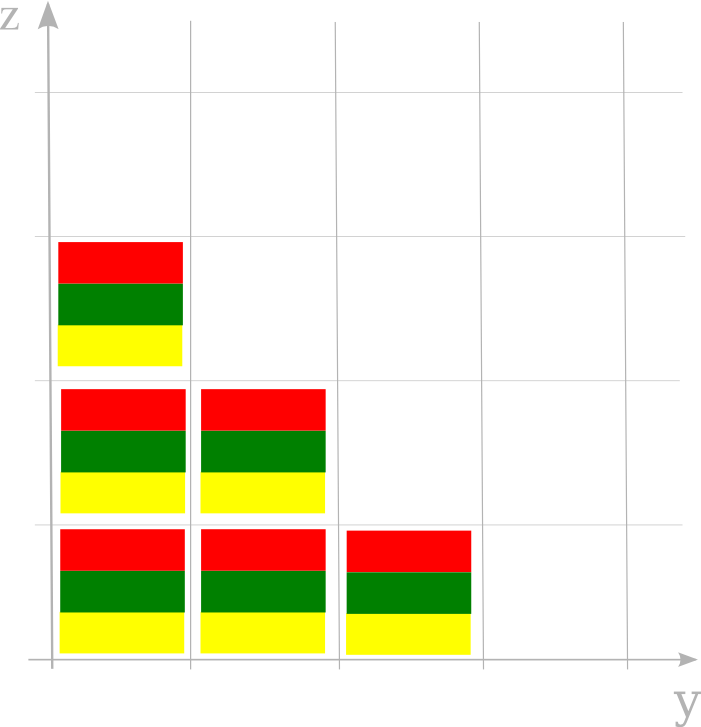
\includegraphics[width=0.29\textwidth]{images/belegung.png}}\hfill
\subfigure[Regalbediengerät]{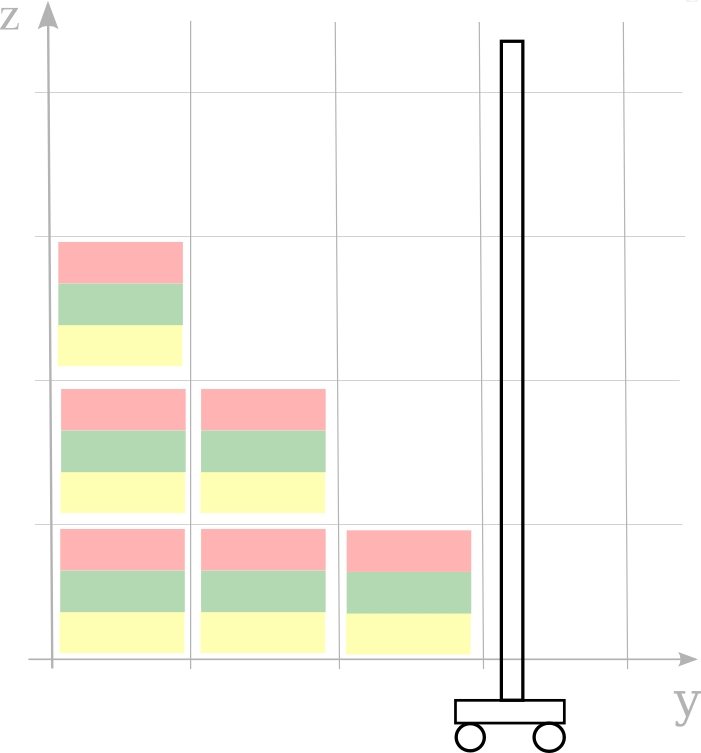
\includegraphics[width=0.29\textwidth]{images/rbg-arm.png}}
\caption{Trennungen}
\end{figure}

\begin{figure}
\subfigure[Regalbediengerät-Ausleger]{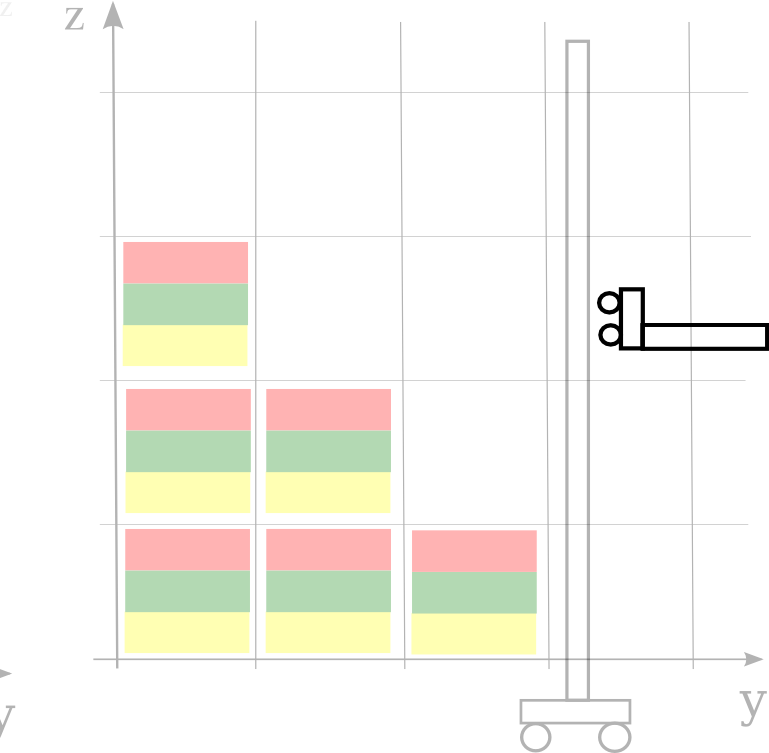
\includegraphics[width=0.29\textwidth]{images/rbg-ausleger.png}}\hfill
\subfigure[Lagergut]{
\includegraphics[width=0.19\textwidth]{images/lagergut.png}}
\caption{Weitere Trennungen}
\end{figure}
%

%EOF


%\section{Sonstiges}

%EOF

\section{Resultate}
Die Ausgabe des Durchlaufs wird in der Konsole ausgeben. Es sind die folgenden Informationen vorhanden:
%
\begin{itemize}
  \item Kompletter Lagerort
  \item Lagerplätze und deren Belegung
  \item Bekannte Jobs beim Simulationsstart
  \item Gewählte Parameter
  \item Neuer Zustand des gesamten Lagerorts
\end{itemize}

\begin{verbatim}
Lagerplatzzuweisung vor Start der Simulation:
---------------------------------------------
Lagerort:
  Name = my location 2
  Anzahl Gassen: 5
    Name: Gasse1, X-Koordinate: 1000, Breite: 1000
    Grid L: Name: Grid1, Tiefe: 1000, Laenge: 20400, Hoehe: 11250
    Grid R: Name: Grid2, Tiefe: 1000, Laenge: 20400, Hoehe: 11250

    Name: Gasse2, X-Koordinate: 4000, Breite: 1000
    Grid L: Name: Grid3, Tiefe: 1000, Laenge: 4800, Hoehe: 1600
    Grid R: Name: Grid4, Tiefe: 1000, Laenge: 4800, Hoehe: 1600

 [snip]

  Anzahl Bin: 710

  1 - ID: Gasse1-0-Grid1-A-1, Artikel:            
          , Koordinaten: (X/Y/Z/U) : 1000/0/0/-1000
  2 - ID: Gasse1-0-Grid1-A-2, Artikel:            
          , Koordinaten: (X/Y/Z/U) : 1000/0/600/-1000
  3 - ID: Gasse1-0-Grid1-A-3, Artikel:            
          , Koordinaten: (X/Y/Z/U) : 1000/0/1400/-1000
  4 - ID: Gasse1-0-Grid1-A-4, Artikel:            
          , Koordinaten: (X/Y/Z/U) : 1000/0/1900/-1000
  5 - ID: Gasse1-0-Grid1-A-5, Artikel:            
          , Koordinaten: (X/Y/Z/U) : 1000/0/2500/-1000
  6 - ID: Gasse1-0-Grid1-A-6, Artikel: Article 828
          , Koordinaten: (X/Y/Z/U) : 1000/0/3250/-1000
  7 - ID: Gasse1-0-Grid1-A-7, Artikel:            
          , Koordinaten: (X/Y/Z/U) : 1000/0/4050/-1000
  8 - ID: Gasse1-0-Grid1-A-8, Artikel: Article 447
          , Koordinaten: (X/Y/Z/U) : 1000/0/4550/-1000
 [snip]
709 - ID: Gasse5-1-Grid10-D-3, Artikel:           
          , Koordinaten: (X/Y/Z/U) : 14000/3200/1000/1000
710 - ID: Gasse5-1-Grid10-D-4, Artikel: Article 1382
          , Koordinaten: (X/Y/Z/U) : 14000/3200/1600/1000

Bereits bekannte Jobs beim Start der Simulation:
------------------------------------------------
Job: ID = '  4', RackFeeder = 'Gasse3', Startzeit = 2000.01.01 00:00:00.049
Job: ID = '  2', RackFeeder = 'Gasse2', Startzeit = 2000.01.01 00:00:00.050
Job: ID = '  3', RackFeeder = 'Gasse3', Startzeit = 2000.01.01 00:00:02.321
[snip]

Erinnerungsevent hinzugefuegt; Eventzeit: 2000.01.01 00:00:00.049
Erinnerungsevent hinzugefuegt; Eventzeit: 2000.01.01 00:00:00.050
[snip]

Simulation wird nun gestartet:
Aktuelle Systemzeit: 2014.01.17 12:48:50.657
Aktueller Faktor: 1.0
Aktueller Modus: AS_FAST_AS_POSSIBLE

---------------------------------------------------
1        -------------------------------------------------
Simulationszeit: 2000:01:01 00:00:00.003
Erinnerungsevent gefunden, Startzeit: 2000.01.01 00:00:00.049

Wartezeit in ms (simuliert): 45

Simulationszeit (echt) nach Wartezeit: 2000:01:01 00:00:00.050
Simulationszeit (soll) nach Wartezeit: 2000.01.01 00:00:00.049

Kein Nachfolgeevent. Eventuell Erinnerungsevents oder Startevents anlegen?
Event hinzugefuegt fuer Job '4', RackFeeder 'Gasse3'; 
  Eventzeit:  2000.01.01 00:00:00.049
-------------------------------------------------
2        ------------------------------------------
Simulationszeit: 2000:01:01 00:00:00.079
[snip]
Wartezeit in ms (simuliert): 0

Simulationszeit (echt) nach Wartezeit: 2000:01:01 00:10:07.744
Simulationszeit (soll) nach Wartezeit: 2000.01.01 00:10:07.740

Kein Nachfolgeevent. Eventuell Erinnerungsevents oder Startevents anlegen?
----------------------------------------------------
Simulation wird nun beendet, Start-Systemzeit: 2014.01.17 12:48:50.657
                          aktuelle Systemzeit: 2014.01.17 12:48:51.140

Vergangene Systemzeit in Millis: 483
\end{verbatim}
Die komplette Ausgabe kann auch in eine Datei geschrieben werden, was einen späteren Vergleich der Durchgänge ermöglicht.

%EOF

%\section{Resultate}

%EOF

\clearpage
%APPENDIX%%%%%%%%%%%%%%%%%%%%%%%%%%%%%%%%%%%%%%%%%
%\pagenumbering{arabic} % Seitennummerierung durch Buchstaben
\appendix
\clearpage
%\addcontentsline{toc}{section}{Anhang}
%\section*{Anhang}

% Abbildungsverzeichnis
\renewcommand{\listfigurename}{}
\section{Abbildungsverzeichnis}
%\addcontentsline{toc}{section}{Abbildungsverzeichnis}
\listoffigures

% Tabellenverzeichis
%\renewcommand{\listtableename}{}
%\section{Tabellenverzeichnis}
%\addcontentsline{toc}{section}{Tabellenverzeichnis}
%\listoftables

% Source location: https://github.com/fabaff/abbreviations-tex
% Released under the BSD license. See LICENSE file for details.
%
% Usage - Verwendung
%
% \ac{KDE}   Gibt bei der ersten Verwendung die Langform mit der Abkürzung in Klammern aus, ab dann stets die Kurzform.
% \acs{KDE}  Gibt die Abkürzung aus.
% \acf{KDE}  Gibt die Langform und die Kurzform aus.
% \acl{KDE}  Gibt nur die Langform ohne die Kurzform aus.
% 
% \acro{}{}
%
\section{Abkürzungsverzeichnis}\label{abbr}
%
\begin{acronym}
%
%
\acro{HRL}{(Paletten-) Hochregallager}
\acro{RBG}{Regalbediengerät}
\acro{LAM}{Lastaufnahmemittel}
\acro{etL}{einfachtiefes Lager}
\acro{dtL}{doppeltiefes Lager}
\acro{dbG}{(doppeltiefes Lager mit) doppelbreitem Lagergang}
%\acro{ÜP}{Übergabepunkt}
%\acro{ÜE}{Aufnahmepunkt}
%\acro{ÜA}{Abgabepunkt}
%\acro{ÜEA}{Übergabepunkt bestehend aus parallel angeordnetem Aufnahme- und Abgabepunkt}
\acro{Lagereinheit}{LE}
%\acro{}{}
%\acro{}{}
%\acro{}{}
%\acro{}{}

\setlength{\itemsep}{-\parsep} %Entfernen des Abstand
\renewcommand{\bflabel}[1]{\normalfont{\normalsize{#1}}\hfill} % Korrektur der Schriftart

%0-9
\acro{1NF}{Erste Normalform (engl. First Normal Form)}
\acro{2NF}{Zweite Normalform (engl. Second Normal Form)}
\acro{3FN}{Dritte Normalform (engl. Third Normal Form)}
\acro{3DES}{Triple Data Encryption Standard}
\acro{3DESEP}{Triple Data Encryption Standard Encryption Protocol}

%A
\acro{A-GPS}{Assisted Global Positioning System}
\acro{AB-EBV}{Ausführungsbestimmungen Eisenbahnverordnung}
\acro{ACL}{Access Control List}
\acro{ACPI}{Advanced Configuration and Power Interface}
\acro{ACS}{Applied Computer Science}
\acro{AD}{Active Directory}
\acro{ADSL}{Asymmetric Digital Subscriber Line}
\acro{ADSP}{AppleTalk Data Stream Protocol}
\acro{AEP}{AppleTalk Echo Protocol}
\acro{AES}{Advanced Encryption Standard}
\acro{AFP}{Apple Filing Protocol}
\acro{AGP}{Accelerated Graphics Port}
\acro{AGU}{Address Generation Unit}
\acro{AHCI}{Advanced Host Controller Interface}
\acro{AMD}{Advanced Micro Devices}
\acro{AMQP}{Advanced Message Queuing Protocol}
\acro{ANSI}{American National Standards Institute}
\acro{AP}{Access Point (Wireless-LAN-Zugangspunkt)}
\acro{APM}{Advanced Power Management}
\acro{APOP}{Authenticated Post Office Protocol}
\acro{ASCII}{American Standard Code for Information Interchange (amerikanische Standardkodierung für den Informationsaustausch)}
\acro{ARP}{Address Resolution Protocol}
\acro{ARPANET}{Advanced Research Projects Agency Network}

%B
\acro{BAKOM}{Bundesamt für Kommunikation}
\acro{Bash}{Bourne-again shell}
\acro{BDSG}{Deutsche Bundesdatenschutzgesetz}
\acro{BGP}{Border Gateway Protocol}
\acro{BIOS}{Basic Input Output System, Firmware bei x86-Systeme}
\acro{BLOB}{Binary Large Object}
\acro{BNC}{Bayonet Neill Concelman}
\acro{BOOTP}{Bootstrap Protocol}
\acro{BSD}{Berkeley Software Distribution}
\acro{BSI}{Bundesamt für Sicherheit in der Informationstechnik}
\acro{BV}{Bundesverfassung}

%C
\acro{CAD}{Computer-Aided Design (Computerunterstütztes Design)}
\acro{CAE}{Computer-aided engineering}
\acro{CAF}{Composite Application Framework}
\acro{CAM}{Computer-aided manufacturing}
\acro{CAN}{Controller Area Network}
\acro{CAS}{Computeralgebrasystem}
\acro{CDATA}{Character Data}
\acro{CDC}{Connected Device Configuration}
\acro{CDE}{Common Desktop Environment}
\acro{CEN}{Europäische Komitee für Normung, franz. Comitée Européen de Normalisation}
\acro{CEPT}{Conférence Européenne des Administrations des Postes et des Télécommunications}
\acro{CF}{CompactFlash}
\acro{CERT}{Computer Emergency Response Team}
\acro{CGI}{Common Gateway Interface}
\acro{CHAP}{Challenge Handshake Authentication Protocol}
\acro{CHS}{Cylinder Head Sector}
\acro{CICS}{Customer Information Control System}
\acro{CIDR}{Classless Inter-Domain Routing}
\acro{CIF}{Common Intermediate Format}
\acro{CIFS}{Common Internet File System}
\acro{CIM}{Computer-integrated manufacturing}
\acro{CMS}{Content-Management-System}
\acro{CPU}{Central processing unit}
\acro{CRC}{Cyclic Redundancy Check}
\acro{CSI}{Common System Interface}
\acro{CUPS}{Common Unix Printing System}
\acro{CVE}{Common Vulnerabilities and Exposures}
\acro{CVS}{Concurrent Versions System}

%D
\acro{DB}{Datenbank}
\acro{DBMS}{Database management system}
\acro{DCE}{Distributed Computing Environment}
\acro{DDL}{Data Definition Language}
\acro{DDoS}{Distributed Denial of Service}
\acro{DEA}{Data Encryption Algorithm}
\acro{DECT}{Digital Enhanced Cordless Telecommunications}
\acro{DENIC}{DE Network Information Center}
\acro{DES}{Data Encryption Standard}
\acro{DH}{Diffie-Hellman}
\acro{DHCP}{Dynamic Host Configuration Protocol}
\acro{DHS}{Department of Homeland Security}
\acro{DIN}{Deutsches Institut für Normung e.V.}
\acro{DLL}{Dynamic Link Library}
\acro{DMA}{Direct Memory Access}
\acro{DMCA}{Digital Millennium Copyright Act}
\acro{DMS}{Dehnungsmessstreifen}
\acro{DMZ}{Demilitarized Zone (Demilitarisierte Zone)}
\acro{DNSBL}{DNS-based Blackhole List}
\acro{DNS}{Domain Name System}
\acro{DoD}{Department of Defense}
\acro{DOM}{Document Object Model}
\acro{DoS}{Denial of Service}
\acro{DRAM}{Dynamic Random Access Memory}
\acro{DSG}{Bundesgesetz über den Datenschutz}
\acro{DSL}{Digital Subscriber Line}
\acro{DUN}{Dial-Up Networking}
\acro{DXF}{Drawing Interchange Format}
\acro{DARPA}{Defense Advanced Research Projects Agency}

%E
\acro{EAI}{Enterprise Application Integration}
\acro{EEC}{European Economic Community}
\acro{EJPD}{Eidgen\"{o}ssisches Justiz- und Polizeidepartement}
\acro{EN}{Europäische Norm}
\acro{EURAMET}{European Association of National Metrology Institutes}
\acro{EWG}{Europäische Wirtschaftsgemeinschaft, auch EEC}
%\acro{EDÖB}{Eidgenössischer Datenschutz- und Öffentlichkeitsbeauftragter}
\acro{Ext2}{Second extended Filesystem}
\acro{ERP}{Enterprise Resource Planning}
\acro{EIDE}{Enhanced IDE}
\acro{EGA}{Enhanced Graphics Array}
\acro{EPROM}{Erasable Programmable Read-Only Memory}
\acro{EEPROM}{Electronically Erasable Programmable Read-Only Memory}
\acro{EBML}{Extensible Binary Meta Language}
\acro{EOF}{End of File}
\acro{EFF}{Electronic Frontier Foundation}
\acro{EISA}{Extended Industry Standard Architecture}
\acro{ESB}{Enterprise Service Bus}
\acro{ESD}{Electrostatic Discharge}

%F
\acro{FAT}{File Allocation Table}
\acro{FDMA}{Frequency Division Multiple Access}
\acro{FE}{Finite Elemente oder auch Finite-Elemente-Methode (FEM)}
\acro{FCC}{Federal Communications Commission}
\acro{FDE}{Full Disk encryption}
\acro{FSB}{Front Side Bus}
\acro{FTP}{File Transfer Protocol}
\acro{FHS}{Filesystem Hierarchy Standard}
\acro{FLOSS}{Free/Libre/Open Source Software}
\acro{FLOSS}{Free and Open Source Software}
\acro{FEM}{Finite Element method}
\acro{FPS}{Floating Point Systems}
\acro{FPGA}{Field Programmable Gate Array}
\acro{FLOPS}{FLoating-Point Operations Per Second}
\acro{FSF}{Free Software Fundation}
\acro{FSM}{Finite State Machine}

%G
\acro{GINA}{Graphical Identification and Authentication}
\acro{GnuPG}{GNU Privacy Guard}
\acro{GPL}{General Public License}
\acro{GPO}{Group Policy Object}
\acro{GPRS}{General Packet Radio Service}
\acro{GPS}{Global Positioning System}
\acro{GRE}{Generic Routing Encapsulation}
\acro{GRUB}{GRand Unified Bootloader}
\acro{GTSM}{Generalized TTL Security Mechanism}
\acro{GUI}{Graphical User Interface}

%H
\acro{HA}{High Availability}
\acro{HHS}{Hacker Highschool}
\acro{HCI}{Host Controller Interface}
\acro{HIP}{Host Identity Protocol}
\acro{HFS}{Hierarchical File System}
\acro{HMI}{Human-Machine Interface}
\acro{HPFS}{High-Performance File System}
\acro{HTCP}{Hyper Text Caching Protocol}
\acro{HTTP}{Hypertext Transfer Protocol}
\acro{HTTPS}{Secure Hypertext Transfer Protocol}
\acro{HHS}{Hacker Highschool}

%I
\acro{I2C}{Inter-Integrated Circuit}
\acro{ICANN}{Internet Corporation for Assigned Names and Numbers}
\acro{ICE}{Intercity-Express}
\acro{IEEE}{Institute of Electrical and Electronics Engineers}
\acro{IETF}{Internet Engineering Task Force}
\acro{IGMP}{Internet Group Management Protocol}
\acro{IGRP}{Interior Gateway Routing Protocol}
\acro{IP}{Internet Protocol}
\acro{IPPP}{ISDN Point-to-Point Protocol}
\acro{IPTV}{Internet-Protokoll-Fernsehen}
\acro{IPX}{Internetwork Packet Exchange}
\acro{IRC}{Internet Relay Chat}
\acro{ISO}{International Standards Organisation}
\acro{ISP}{Internet Service Provider}

%K
\acro{KB}{Knowledge Base}
\acro{KDE}{K Desktop Environment}
\acro{KDC}{Kerberos Key Distribution Center}
\acro{KEK}{Key Encryption Key}
\acro{KGD}{Key generation and distribution}
\acro{KINK}{ Kerberized Internet Negotiation of Keys}
\acro{KSG}{Key Stream Generator}
\acro{KSK}{Key Signing Key}

%L
\acro{L2CAP}{Logical Link Control and Adaptation Protocol}
\acro{L2F}{Layer 2 Forwarding}
\acro{L2TP}{Layer 2 Tunneling Protocol}
\acro{L2VPN}{Layer 2 Virtual Private Network}
\acro{LAN}{Local Area Network}
\acro{LCD}{Liquid Crystal Display}
\acro{LDA}{Local Delivery Agent}
\acro{LDAP}{Lightweight Directory Access Protocol}
\acro{LED}{Light Emitting Diode}
\acro{LIR}{Local Internet Registry}
\acro{LMP}{Link Manager Protocol}
\acro{LRA}{Local Registration Authority}
\acro{LSA}{Local Security Authority}
\acro{LUA}{Limited User Account}
\acro{LXDE}{Lightweight X11 Desktop Environment}

%M
\acro{MAN}{Metropolitan Area Network}
\acro{MAPI}{Messaging Application Programming Interface}
\acro{MAU}{Multistation Access Unit}
\acro{MBR}{Master Boot Record}
\acro{METAS}{Bundesamt für Metrologie und Akkreditierung}
\acro{MFM}{Modified Frequency Modulation}
\acro{MFT}{Master File Table}
\acro{MIME}{Multipurpose Internet Mail Extensions}
\acro{MIS}{Management Information Systems}
\acro{MMV}{Messmittelverordnung}
\acro{MPI}{Message Passing Interface}
\acro{MPLS}{Multiprotocol Label Switching}
\acro{MPP}{Massively Parallel Processing}
\acro{MSB}{Most Significant Bit}
\acro{MSDN}{Microsoft Developer Network}
\acro{MSN}{Microsoft Network}
\acro{MTU}{Maximum Transmission Unit}
\acro{MUA}{Mail User Agent}
\acro{MX}{Mail Exchange}
\acro{MIPS}{Microprocessor without Interlocked Pipeline Stages oder Million Instructions Per Second}
\acro{MIB}{Management Information Base}
\acro{MAC}{Mandatory Access Control}
\acro{MAPI}{Messaging Application Programming Interface}
\acro{MANET}{Mobile Ad-Hoc Network}

%N
\acro{NAT}{Network Address Translation}
\acro{NCP}{Network Control Program}
\acro{NDIS}{Network Driver Interface Specification}
\acro{NDPS}{Novell Distributed Print Services}
\acro{NDS}{Novell Directory Services}
\acro{NEDC}{New Enterprise Data Center}
\acro{NCSA}{National Center for Supercomputing Applications}
\acro{NFC}{Near field communication}
\acro{NFS}{Network File System}
\acro{NIC}{Network Information Center oder Network Interface Card}
\acro{NIST}{National Institute of Standards and Technology}
\acro{NNTP}{Network News Transfer Protocol}
\acro{NOC}{Network Operation Center}
\acro{NSA}{National Security Agency}
\acro{NSF}{National Science Foundation}
\acro{NSFNET}{National Science Foundation Network}
\acro{NTFS}{New Technology File System}
\acro{NTP}{Network Time Protocol}
\acro{NTSC}{National Television Standards Committee}
\acro{NUI}{Natural User Interface}
\acro{NUMA}{Non-Uniform Memory Access}
\acro{NVD}{National Vulnerability Database}
\acro{NVE}{Networked Virtual Environment}
\acro{NVRAM}{Non Volatile Random Access Memory}
\acro{NYSE}{New York Stock Exchange}

%O
\acro{OHCI}{Open Host Controller Interface}
\acro{OIML}{Internationale Organisation für das gesetzliche Messwesen (engl. International Organization of Legal Metrology)}
\acro{OLAP}{Online Analytical Processing}
\acro{OLED}{Organic Light Emitting Diode}
\acro{OLE}{Object Linking and Embedding}
\acro{OLSR}{Optimized Link State Routing}
\acro{OODBMS}{Object-Oriented DataBase Management System}
\acro{OOo}{OpenOffice.org}
\acro{OOP}{Objektorientierte Programmierung}
\acro{OR}{Obligationenrecht}
\acro{OSA}{Open Systems Architecture}
\acro{OSGi}{Open Services Gateway Initiative}
\acro{OSI}{Open Systems Interconnection}
\acro{OS}{Operating System}
\acro{OSPF}{Open Shortest Path First}
\acro{OSSTMM}{Open Source Security Testing Methodology Manual}
\acro{OWASP}{Open Web Application Security Project}

%P
\acro{PAM}{Pluggable Authentication Module}
\acro{PAN}{Personal Area Network}
\acro{PCIe/PCI-E}{Peripheral Component Interconnect Express}
\acro{PCI}{Peripheral Component Interconnect}
\acro{PCI-X}{Peripheral Component Interface Extension}
\acro{PCMCIA}{Personal Computer Memory Card International Association}
\acro{PC/SC}{Personal Computer/Smart Card}
\acro{PGP}{Pretty Good Privacy}
\acro{PIO}{Programmed Input/Output}
\acro{PKI}{Public Key Infrastructure}
\acro{PLA}{Programmable Logic Array}
\acro{PPPoE}{PPP over Ethernet}
\acro{PPP}{Point-to-Point Protocol}
\acro{PPTP}{Point-to-Point Tunneling Protocol}
\acro{PPU}{Physics Processing Unit}
\acro{PSTN}{Public Switched Telephone Network}
\acro{PTES}{Penetration Testing Execution Standard}
\acro{PVC}{Permanent Virtual Circuit}
\acro{PWM}{Pulse Width Modulation}
\acro{PXE}{Preboot Execution Environment}

%Q
\acro{QPI}{QuickPath Interconnect}
\acro{QoS}{Quality of Service}

%R
\acro{RAD}{Rapid Application Development}
\acro{RAID}{Redundant Array of Independent Disks, ursprünglich Redundant Array of Inexpensive Disks}
\acro{RADIUS}{Remote Authentication Dial-In User Service}
\acro{RAM}{Random Access Memory}
\acro{RAR}{Resource Adapter}
\acro{RARP}{Reverse Address Resolution Protocol}
\acro{RAS}{Remote Access Service}
\acro{RAV}{Risk Assessment Values}
\acro{RBL}{Realtime Blackhole List}
\acro{RDBMS}{Relational Database Management System}
\acro{RDF}{Resource Description Framework}
\acro{RDP}{Remote Desktop Protocol}
\acro{RED}{Random Early Detection}
\acro{REST}{Representational State Transfer}
\acro{RIA}{Rich Internet Application}
\acro{RIMM}{Rambus In-Line Memory Modul}
\acro{RIP}{Routing Information Protocol}
\acro{ROM}{Read Only Memory}
\acro{RPC}{Remote Procedure Call}
\acro{RSA}{Rivest, Shamir, Adleman}
\acro{RSH}{Remote Shell}
\acro{RSS}{Really Simple Syndication}
\acro{RTC}{Real Time Clock}
\acro{RTF}{Rich Text Format}
\acro{RTFM}{Read The Fucking Manual}
\acro{RTL}{Register Transfer Level (Ebene in Hardware / Hardware-Modellierung)}
\acro{RTOS}{Realtime Operating System}
\acro{RTP}{Realtime Transport Protocol}
\acro{RTSI}{Real Time System Integration}
\acro{RTTI}{Runtime Type Information}

%S
\acro{SAA}{Systems Application Architecture}
\acro{SACD}{Super Audio Compact Disc}
\acro{SAFT}{Simple Asynchronous File Transfer}
\acro{SAM}{Security Account Manager}
\acro{SAN}{Storage Area Network}
\acro{SASL}{Simple Authentication and Security Layer}
\acro{SAS}{Serial Attached SCSI}
\acro{SATA}{Serial ATA}
\acro{SATL}{SCSI/ATA Translation Layer}
\acro{SAT}{SCSI/ATA Translation}
\acro{SCARE}{Source Code Analysis Risk Evaluation}
\acro{SCSI}{Small Computer System Interface}
\acro{SDF}{Synchronous Data Flow}
\acro{SDH}{Synchronous Digital Hierarchy}
\acro{SELinux}{Security-Enhanced Linux}
\acro{SGML}{Standard Generalized Markup Language}
\acro{SHFS}{Shell File System}
\acro{SHTTP}{Secure Hyper Text Transport Protocol}
\acro{SIA}{Schweizerischer Ingenieur- und Architektenverein}
\acro{SIMD}{Single Instruction Multiple Data}
\acro{SIMM}{Single Inline Memory Module}
\acro{SIM}{Subscriber Identity Module}
\acro{SIP}{Session Initiation Protocol}
\acro{SMB}{System Management Bus}
\acro{S/MIME}{Secure / Multipurpose Internet Mail Extensions}
\acro{SMP}{Symmetric Multi-Processing, siehe Symmetrisches Multiprozessorsystem}
\acro{SMS}{Short Message Service}
\acro{SMTP}{Simple Mail Transfer Protocol}
\acro{SMT}{Simultaneous Multithreading}
\acro{SN}{Schweizer Norm; siehe Schweizerische Normen-Vereinigung}
\acro{S/N}{Serial Number}
\acro{SOK}{Schienenoberkante}
\acro{SOMA}{Security Operations Maturity Architecture}
\acro{SQL}{Structured Query Language}
\acro{SR}{Ständerat des Schweizer Parlament}
\acro{SSD}{Solid-State-Drive}
\acro{SSE}{Streaming SIMD Extensions}
\acro{SSH}{Secure Shell}
\acro{SSID}{Service Set Identifier}
\acro{SSI}{Server Side Includes}
\acro{SSL}{Secure Sockets Layer, alte Bezeichnung für Transport Layer Security}
\acro{STAR}{Security Test Audit Report}

%T
\acro{TCP}{Transmission Control Protocol}
\acro{TCPA}{Trusted Computing Platform Alliance}
\acro{TCP/IP}{Transmission Control Protocol / Internet Protocol}
\acro{TDMA}{Time Division Multiple Access}
\acro{TFT}{Thin Film Transistor}
\acro{TFTP}{Trivial File Transfer Protocol}
\acro{TIPC}{Transparente Inter-Process Communication}
\acro{TLB}{Translation Lookaside Buffer}
\acro{TLD}{Top-Level-Domain oder Tag Library Descriptor}
\acro{TLM}{Transaction Level Modelling}
\acro{TLS}{Transport Layer Security}
\acro{TM}{Transactional Memory}
\acro{TGV}{französische Hochgeschwindigkeitszugskonzept, Train a grande vitesse}
\acro{TTL}{Time To Live}

%U
\acro{UAC}{User Account Control}
\acro{UART}{Universal Asynchronous Receiver Transmitter}
\acro{UAT}{User Acceptance Test}
\acro{UBE}{Unsolicited Bulk Email}
\acro{UCD}{User Centered Design}
\acro{UCE}{Unsolicited Commercial E-Mail}
\acro{UCP}{Universal Computer Protocol}
\acro{UCS}{Universal Character Set}
\acro{UDF}{User Defined Function}
\acro{UDMA}{Ultra-Direct Memory Access}
\acro{UDP}{User Datagram Protocol}
\acro{UEFI}{Unified Extensible Firmware Interface}
\acro{UML}{Unified Modeling Language}
\acro{UMTS}{Universal Mobile Telecommunications System}
\acro{UPnP}{Universal Plug and Play}
\acro{UPS}{Uninterruptible Power Supply}
\acro{URI}{Uniform Resource Identifier}
\acro{URL}{Uniform Resource Locator}
\acro{URN}{Uniform Resource Name}
\acro{USB}{Universal Serial Bus}
\acro{USV}{Unterbrechungsfreie Stromversorgung}
\acro{UI}{User Interface}
\acro{UUID}{Universally Unique Identifier}

%V
\acro{VDSG}{Verordnung zum Bundesgesetz über den Datenschutz}
\acro{VDI}{Verein Deutscher Ingenieure (engl. Association of German Engineers)}
\acro{VFS}{Virtual Filesystem Switch}
\acro{VESA}{Video Electronics Standards Association}
\acro{VLAN}{Virtual Local Area Network}
\acro{VLB}{VESA Local Bus}
\acro{VLIW}{Very Long Instruction Word}
\acro{VLSI}{Very Large Scale Integration}
\acro{VM}{Virtuelle Maschine}
\acro{VMS}{Virtual Memory System}
\acro{VNC}{Virtual Network Computing}
\acro{VoIP}{Voice over IP}
\acro{VRAM}{Video Random Access Memory}
\acro{VRML}{Virtual Reality Modeling Language}
\acro{VRRP}{Virtual Router Redundancy Protocol}
\acro{VPN}{Virtual private network, virtuelles privates Netz}
\acro{VSAM}{Virtual Storage Access Method}

%W
\acro{WDS}{Wireless Distribution System}
\acro{WEP}{Wired Equivalent Privacy}
\acro{WINS}{Windows Internet Naming Service}
\acro{WISP}{Wireless Internet Service Provider}
\acro{WLAN}{Wireless Local Area Network}
\acro{WWAN}{Wireless Wide Area Network}
\acro{WWW}{World Wide Web}
\acro{WELMEC}{European cooperation in legal metrology}
\acro{WPA}{Wi-Fi Protected Access}
\acro{WPAN}{Wireless Personal Area Network}
\acro{WebDAV}{WWW Distributed Authoring and Versioning}

%X
\acro{XAML}{eXtensible Application Markup Language}
\acro{XAMPP}{Extended Apache/MySQL/PHP/Perl}
\acro{XGA}{Extended Graphics Array}
\acro{XML}{Extensible Markup Language}
\acro{XML-RPC}{Extensible Markup Language Remote Procedure Call}
\acro{XMPP}{Extensible Messaging and Presence Protocol}
\acro{XMS}{Extended Memory Specification}
\acro{XMSF}{Extensible Modeling and Simulation Framework}
\acro{XOG}{XML Open Gateway}
\acro{XrML}{Extensible rights Markup Language}
\acro{XSD}{XML Schema Definition}
\acro{XSL}{Extensible Stylesheet Language}
\acro{XSL-FO}{Extensible Stylesheet Language – Formatting Objects}
\acro{XSLT}{XSL Transformation}
\acro{XSS}{Cross-Site Scripting}

%Y
\acro{Y2K}{Year Two Thousand}
\acro{YAAF}{Yet Another Application Framework}
\acro{YACC}{Yet Another Compiler Compiler}
\acro{YAML}{YAML Ain't Markup Language}
\acro{YP}{Yellow Pages}

%Z
\acro{ZBR}{Zone Bit Recording}
\acro{ZF}{Zero flag}
\acro{ZFS}{Zettabyte File System}
\acro{ZCS}{Zero Code Suppression}
\acro{ZIF}{Zero Insertion Force}
\acro{ZMA}{Zone Multicast Address}
\acro{ZOPE}{Z Object Publishing Environment}
\acro{ZPL}{Z-level Programming Language}
\end{acronym}
%
%EOF


%% Literaturverzeichnis
%
\bibliographystyle{alpha} %Oder für kurze Berichte plain
%\bibliography{literature}
%EOF

\section{Projekt-Beteiligte}
%
%Verfasser
\subsection*{Verfasser}

\begin{tabular}{p{0.5\linewidth}p{0.5\linewidth}}
  & Marc Schärer \href{mailto:scham36@bfh.ch}{\nolinkurl{scham36@bfh.ch}} \\
  & Arthur van Ommen \href{mailto:vanoa1@bfh.ch}{\nolinkurl{vanoa1@bfh.ch}}\\
  & Fabian Affolter \href{mailto:affof11@bfh.ch}{\nolinkurl{affof1@bfh.ch}}\\
\end{tabular}

%
\subsection*{Betreuer}
\begin{tabular}{p{0.5\linewidth}p{0.5\linewidth}}
Berner Fachhochschule &  Jürgen Eckerle \\
Technik und Informatik &  \\
Wankdorffeldstrasse 102 & \\
3014 Bern & \href{mailto:erj1@bfh.ch}{\nolinkurl{erj1@bfh.ch}} \\
\end{tabular}
%
\section{Weiteres}
\subsection*{Differenzierung zwischen Mann und Frau}
Für eine bessere Lesbarkeit bei allgemeinen Aussagen wird nur die männliche Form des Substantivs verwendet. Die Leserinnen bitten die Autoren um Verständnis für diese Vereinfachung.
%
%Trademarks
\subsection*{Markennamen und Warenzeichen}
Alle Markennamen, Warenzeichen und eingetragenen Warenzeichen, die in diesem Dokument verwendet werden, sind Eigentum ihrer rechtmässigen Eigentümer. Sie dienen hier nur der Beschreibung beziehungsweise der Identifikation der jeweiligen Firmen, Produkte und Dienstleistungen.
%EOF

%\documentclass[11pt,a4paper]{article}
\usepackage[paper=a4paper,left=25mm,right=20mm,top=30mm,bottom=30mm]{geometry} 
\usepackage[english, ngerman]{babel}
\usepackage[utf8]{inputenc}
\usepackage[colorlinks=false]{hyperref}
\usepackage[table,usenames,dvipsnames]{xcolor}
\usepackage{tabularx}
\usepackage{graphicx}
\usepackage{listings}
\usepackage{float}
\usepackage{hyperref}
\usepackage{multicol}
\usepackage{fancyhdr}
\usepackage{sectsty}
\usepackage[final]{pdfpages}
%\usepackage{gitinfo}
%\usepackage{totpages}
\usepackage{datetime}
\usepackage{subcaption}
%\usepackage[printonlyused]{acronym}
%\usepackage[toc]{glossaries}

%Definitionen
\includepdfset{pages=-} %Alle Seite importieren  Option: noautoscale
\setlength{\parindent}{0em} %Einrueckung eines neuen Absatzes, 0 keine Einrueckung

\definecolor{rowc1}{RGB}{40,75,95}

\setcounter{tocdepth}{3}
\setcounter{secnumdepth}{3}

\ifpdf
\pdfinfo {
	/Author (Marc Schärer, Arthur van Ommen, Fabian Affolter)
	/Title (Report)
	/Subject ()
	/Keywords ()
	/CreationDate (D:\pdfdate)
}
\fi

\pagestyle{fancy}
\renewcommand{\headrulewidth}{0pt}
\lhead{}%\includegraphics[width=80mm]{logo.png}}
\chead{}
\rhead{}
\lfoot{}
\cfoot{\thepage}
\rfoot{}

\renewcommand{\arraystretch}{1.3}
\lstset{basicstyle=\ttfamily,breaklines=true}

\begin{document}
%%%%%%%%%%%%%%%%%%%%%%%%%%%%%%%%%%%%%%%%%%%%%%%%%
{\huge \textbf{Anforderungs-Dokumentation}} - \textbf{Hochregallager} \\
\tableofcontents

\section{Vorwort}
%
\subsection{Zielgruppe}
Dieses Dokument beschreibt die Anforderungen an eine Software-Lösung für die Simulation und Optimierung von Hochregallagern im Detail. Es enthält die Aspekte der gesuchten Lösung mit dem Fokus, welcher auf die technische Seite gerichtet ist. Der Leser sollte ein grundlegendes Verständnis von Logistik und Lagerungssystem haben und mit der in diesem Bereich verwendeten Terminologie vertraut sein. 
%
\subsection{Autoren}
Die Autoren diesen Dokument sind:
%
\begin{itemize}
  \item Marc Schärer \href{mailto:scham36@bfh.ch}{\nolinkurl{scham36@bfh.ch}}
  \item Arthur van Ommen \href{mailto:vanoa1@bfh.ch}{\nolinkurl{vanoa1@bfh.ch}}
  \item Fabian Affolter \href{mailto:affof11@bfh.ch}{\nolinkurl{affof1@bfh.ch}}
\end{itemize}
%
\subsection{Dokument-Versionen}

\begin{table}[h]
  %\caption{}
  %\label{tab:releases}

  \begin{center}
    \begin{tabular}{|c|c|c|c|}
      \hline
      \textbf{Version} & \textbf{Autor} & \textbf{Bemerkungen} & Datum\\
      \hline
      0 & Team & Skelett & 20.09.2013\\
      0.1 & Team & erste Version, Dokumentation der Anforderungen &  27.09.2013 \\
      0.2 & Team & überarbeitete Version, Prioritätenliste, Schwerpunkte, u. a. & 01.10.2013 \\
      \hline
    \end{tabular}
  \end{center}
\end{table}
%
%\subsection{Glossar}
%tbd
%
\section{Einleitung}
Ein Hochregallager (HRL) beschreibt ein Lagersystem mit Plätzen in sogenannten Regalen. Hochregallager gibt ein in den unterschiedlichsten Ausprägungen. Die grössten Ausführungen besitzen Höhen bis etwa 50 m und können mehreren hunderttausend Plätze besitzen. Oftmals werden direkt Euro-Paletten als Träger für das Lagergut verwendet, ist das Lagergut zu klein, werden häufig spezielle Kunststoff-Behälter benutzt.\\
Grobgesagt besteht ein Hochregallager aus einer bestimmten Anzahl von Gassen. Eine Gasse wiederum hat links und rechts Lagerplätze und im Freiraum bewegt sich ein Bediengerät. In einem manuellen Hochregallager ist dieser Raum so gross, dass mit einem Gabelstapler zwischen den Regalwänden manövriert werden kann. Bei automatischen Lagern fährt ein Bediengerät, welches von einem Lagerverwaltungssystem seine Befehle bekommt, ohne manuelle Interventionen in der Gasse und liefert das Lagergut zur Entnahmestelle.\\
Die Hochregallager haben eine hohe Raumnutzung und bei der Erstellung sind hohe Investitionen nötig, da bei kleiner Ausführungen eine Halle um das Hochregallager gebaut werden muss. Bei grossen Varianten wird das Hochregal als Tragstruktur für das Gebäude mitbenutzt. 
%
\section{Benutzeranforderungen}
%
\subsection{Funktionale Anforderungen}
\begin{itemize}
  \item Definition des Szenarios (Statische Parameter)
  \item Eingeben der Simulationsparameter (dynamische Parameter)
  \item Simulationssteuerung
  \item Szenarienmanagement
\end{itemize}
%
\subsection{Nichtfunktionale Anforderungen}
\begin{itemize}
  \item Keine unsinnig grossen (langlaufende) Simulationen
  \item Grafische Darstellung während der Simulation (informativ)
  \item Sprache der Applikation ist in Englisch
  \item Ausgabe / Export der Ergebnisse auf Drucker oder als Dokument (z.B. .txt, .csv, .xml, usw.)
\end{itemize}

%
\subsubsection{Domainspezifische Anforderungen}
\begin{itemize}
  \item Gefahrengut / Brandschutz
  \item Konformität
  \item Arbeitssicherheit
\end{itemize}
%
\section{System-Architektur}
\begin{itemize}
  \item Clientanwendung
  \item Trennung von Simulation, Auswertung und Visualisierung
\end{itemize}
%
\section{Systemanforderungen}
%
\subsection{Funktionale Anforderungen}
\begin{itemize}
  \item Szenario laden
  \item Szenario simulieren / berechnen
  \item Simuliertes Szenario auswerten / ausgeben
%  \item 
%  \item 
\end{itemize}
%
\subsection{Nichtfunktionale Anforderungen}
\begin{itemize}
  \item Lauffähig auf Standard-Hardware
  \item Nur Standard-Software (JRE, Bibliotheken, etc.)
%  \item 
%  \item 
\end{itemize}
%
\section{System-Evolution}
N/A
%
\section{Testing}
\begin{itemize}
  \item Unit tests
%  \item 
%  \item 
%  \item 
\end{itemize}
%
\section{Mögliche Szenarien}
Dieser Abschnitt beschreibt mögliche Szenarien, welche in Simulationen betrachtet werden könnten.
%
\begin{itemize}
  \item Maschinenbaufirma im 1-Schichtbetrieb mit Fertigung / Montage / Service -- kurze Zugriffszeiten Tagsüber, freie Ressourcen während der Nacht
  \item Versandhandel im 3-Schichtbetrieb mit Bereitstellung / Konvektionierung --  hoher Lagerdurchsatz, 24h-Zugriff für Ein-/Auslagerung
  \item Gleichzeitiges Ein-/Auslagern, Queue
  \item Mehrere Ein-/Ausgabeplätze pro Gasse (auf z-Achse)
  \item Mehrere Regalbediengeräte pro Gasse (auf x-Achse, bei mehreren Ein-/Ausgabeplätzen auch auf z-Achse)
  \item Mehrere Ladearme pro Regalbediengerät (mehrere vertikal, horizontal [ohne / mit Durchreichemöglichkeit], radial)
  \item Vorgezogenes Auslagern (Bereitstellung noch im Lager)
  \item Ausfall einer Gasse, Mehrplatzeinlagerung gleicher Teile in unterschiedlichen Gassen
  \item Fixe Lagerplatzzuordnung (Reservation, defekte Lagerplätze, abgeschottete Lagerplätze für Gefahrengut)
  \item Befüllung (inital von leerem Lager / Nachbefüllung) (zufällig chaotisch, zeitoptimiert chaotisch, zugeordnet, positionsoptimiert [ABC])
  \item Optimierung von bereits belegtem Lager aufgrund Zugriff-History
%  \item 
\end{itemize}
%
\section{Schwerpunkte}
\begin{itemize}
  \item Simulation / Simulationsauswertung / Simulationsvisualisierung
  \item Optimierung
\end{itemize}
%
\section{Möglicher Ablauf der Arbeitsschritte}

\begin{enumerate}
  \item Laden eines einfachen Szenarios (mit fixen Einstellungen)
  \item Berechnung der Simulations-Eckdaten
  \item Visuelle Darstellung des Szenario (2D) -- Überprüfung des Klassen-Diagramm, Abschätzung der Performance
  \item Steigerung der Komplexität der Szenarien (einfache Input-Funktion, ASCII- oder Spreadsheet-Datei) -- Szenarien-Management
  \item Simulierte Szenarien auswerten / einfache Daten-Ausgabe
  \item Optimierung von einzelnen Szenarien (nach einer vorgegebenen Auswertung, nach vorgebener Strategie, Änderung der Hochregallager-Parameter)
  \item Erweiterung der Export-Funktion (Spreadsheet oder ähnlich, für grafische Auswertungen)
  \item Erweiterung der visuellen Repräsentation (3D)
  \item Ausgabe für die Dimensionierung/Auslegung von Hochregallagern
  \item Einbezug der Vorzone in Simulation/Optimierung
  \item Multifunktionale Benutzeroberfläche für die Eingabe/Simulation/Auswertung/Auslegung
\end{enumerate}
%
\section{Sonstiges}
\begin{itemize}
  \item Repository: \href{https://github.com/fabaff/high-rack-warehouse}{https://github.com/fabaff/high-rack-warehouse}
  \item Dokumentation: \href{https://github.com/fabaff/high-rack-warehouse/tree/master/docs}{/docs}
  \item Code: \href{https://github.com/fabaff/high-rack-warehouse/}{Pfad momentan unbestimmt}
\end{itemize}
%%%%%%%%%%%%%%%%%%%%%%%%%%%%%%%%%%%%%%%%%%%%%%%%%%%
\end{document}

%\section{Sonstiges}
%
% \subsection*{Dokument-Informationen}
% %
% \rowcolors{1}{white}{white}
% \begin{tabular}{ll}
% Autor: & \authorshort \\
% Original-Dateiname: & \jobname.tex  (Master)\\
% Total Seiten: &  \ref*{TotPages} \\
% Build-Zeitstempel: &  \today, \currenttime \\
% Git tag: & 1.0 \\
%  & \\
% Vollständiger Hash: & \gitHash \\
% Abgekürzter Hash:  & \gitAbbrevHash \\
%  & \\
% \begin{tabular}{l}
% Letzte Commits  \\
%  \\
% \end{tabular}
% &
% \begin{tabular}{llll}
% Autor: & \gitAuthorName & \gitAuthorEmail & \gitAuthorDate \\
% Commiter: & \gitCommitterName & \gitCommitterEmail & \gitCommitterDate \\
% \end{tabular}
% \\
% \end{tabular}
%
%Gender
\subsection*{Differenzierung zwischen Mann und Frau}
Für eine bessere Lesbarkeit bei allgemeinen Aussagen wird nur die männliche Form des Substantivs verwendet. Die Leserinnen bitten die Autoren um Verständnis für diese Vereinfachung.
%
%Trademarks
\subsection*{Markennamen und Warenzeichen}
Alle Markennamen, Warenzeichen und eingetragenen Warenzeichen, die in diesem Dokument verwendet werden, sind Eigentum ihrer rechtmäßigen Eigentümer. Sie dienen hier nur der Beschreibung beziehungsweise der Identifikation der jeweiligen Firmen, Produkte und Dienstleistungen.


%%%%%%%%%%%%%%%%%%%%%%%%%%%%%%%%%%%%%%%%%%%%%%%%%%%%%%%%%%%%%%%
%Index des Dokumentes
%\printindex
%%%%%%%%%%%%%%%%%%%%%%%%%%%%%%%%%%%%%%%%%%%%%%%%%%%
\end{document}
